\documentclass[a4paper,12pt]{article}
\usepackage{mathtools}
\usepackage{graphicx}
%\graphicspath{ {/home/raghavsg/Downloads/grace/photos_n/} }
\newcommand\tab[1][1cm]{\hspace*{#1}}
\usepackage{hyperref}

\usepackage[utf8]{inputenc}

\usepackage{amsmath}
\begin{document}


%\includegraphics[scale=.44]{grace1}
\newpage
\section*{\centerline{Stochastic Filtering of} \centerline{GRACE Mission Data}}
\section{Introduction to GRACE Mission}
 The gravity recovery and climate experiment (grace) satellite mission was launched
on the 17 th of March in 2002 as a joint partnership between the National Aeronautics
and Space Administration (NASA) and the Deutsches Zentrum für Luft- und Raumfahrt
(DLR). Furthermore, it is the second mission under the NASA Earth System Science
Pathfinder (ESSP) program. The mission was originally intended to last for five years,
but is still in orbit.


As variations in the gravity field impacts on both satellites at different times, such
deviations cause a change in the inter-satellite range, which is measured with very high
accuracy from the K-band measurement unit. The measured inter-satellite range can
be transformed into changes in the Earth’s gravity field (Han, 2003), which is described
with the Stokes coefficients Clm and Slm.


\paragraph{Grace Mission} 
The GRACE mission was selected as the second mission under the NASA Earth System Science Pathfinder (ESSP) Program in May 1997. Launched in March of 2002, the GRACE mission is accurately mapping variations in Earth's gravity field. Designed for a nominal mission lifetime of five years, GRACE is currently operating in an extended mission phase, which is expected to continue through at least 2019.

GRACE consists of two identical spacecraft that fly about 220 kilometers (137 miles) apart in a polar orbit 500 kilometers (310 miles) above Earth. GRACE maps Earth's gravity field by making accurate measurements of the distance between the two satellites, using GPS and a microwave ranging system. It is providing scientists from all over the world with an efficient and cost-effective way to map Earth's gravity field with unprecedented accuracy. The results from this mission are yielding crucial information about the distribution and flow of mass within Earth and its surroundings.

The gravity variations studied by GRACE include: changes due to surface and deep currents in the ocean; runoff and ground water storage on land masses; exchanges between ice sheets or glaciers and the ocean; and variations of mass within Earth. Another goal of the mission is to create a better profile of Earth's atmosphere. GRACE results are making a huge contribution to the goals of NASA's Science Mission Directorate, Earth Observation System (EOS) and global climate change studies.
\newpage

%\includegraphics[scale=0.42]{grace2}

%\\
A simplified example of how the distance between the GRACE-FO satellites changes as they pass from the Caribbean Sea across Colombia and Peru (which have higher mass than the oceans) to the Pacific Ocean. Panel 1: When both spacecraft are over the ocean, the distance between them is relatively constant. 
A simplified example of how the distance between the GRACE-FO satellites changes as they pass from the Caribbean Sea across Colombia and Peru (which have higher mass than the oceans) to the Pacific Ocean.

Panel 1: When both spacecraft are over the ocean, the distance between them is relatively constant.

Panel 2: When the leading spacecraft encounters land, the land's higher gravity pulls it away from the trailing spacecraft, which is still over water.

Panel 3: Once the second satellite also encounters the land, it too is pulled toward the higher mass and consequently toward the leading spacecraft. As the lead spacecraft moves past the denser land mass, it is pulled back slightly by the higher gravity of the land.

Panel 4: When both spacecraft are over water again, the trailing spacecraft is slowed by land before returning to its original distance behind the leading spacecraft.





\newpage

\section{Potential Fields}
\begin{itemize}
\item They are conservative (path independent fields) in nature.     
\item Also known as Harmonics.
\end{itemize}
\paragraph{Harmonics:-} 
 
\begin {equation}
\nabla ^2V(r,\theta ,\varphi) = \left( {\underbrace {\frac{\partial ^2V }{\partial r^2} +
\frac{2}{r}\frac{\partial V }{\partial
r}}_{\frac{1}{^{r^2}}\frac{\partial }{\partial r}\left( {r^2\frac{\partial
V }{\partial r}} \right)} + \frac{1}{r^2\sin \theta }\frac{\partial
}{\partial \theta }\left( {\sin \theta \frac{\partial V }{\partial \theta
}} \right) + \frac{1}{r^2\sin ^2\theta }\frac{\partial ^2V }{\partial
\varphi ^2}} \right)
\end{equation}

\begin {equation}
\nabla ^2V(r,\theta ,\varphi) = 0
\end{equation}

\paragraph{Basic Question:-} How do we arrive at this equation??

we have our gravitational potential .i.e. $V(\phi,\lambda,r)$

Gravitational Force is derivative of V and derivative of Gravitational force should be equal to zero and this gives us the following Homogeneous 2nd degree Partial Differential Equation .i.e

   \[ \left( \frac{\partial^2 V}{\partial x^2}
      + \frac{\partial^2 V}{\partial y^2}
      + \frac{\partial^2 V}{\partial z^2} \right)=0 \]

This Homogeneous PDE  can be solved by Method of variable separation and the solution of this is Spherical Harmonics in spherical coordinates i.e.

\begin{equation}
V(\phi,\lambda,r)=\frac{GM}{r}\sum_{l=0}^{\infty} \left(\frac{R}{r}\right)^{l+1}\sum_{m=0}^{l} \widetilde{P}_{lm}(\cos\theta)(\Delta\widetilde{C}_{lm}\cos m\lambda + \Delta\widetilde{S}_{lm}\sin m\lambda)
\end{equation}

\paragraph{Important Functions:} 
In the given equation P is Legendre function and the accompanying combination of sine and cosine function forms the fourier series. So, by looking at this simplified equation of gravity field, one can deduce that other things are merely constants and the gravity fields is combination of Legendre and Trigonometric functions.
These functions i.e. Legendre and trigonometric function also known as fourier functions are Orthogonal to each other. This is the property which helps in Stochastic filtering of raw data in the form of coefficients$ S_{lm}$ and $C_{lm} $which are discussed as follows:  
\paragraph{Stochastic Coefficients:} 
Here, the constant appearing $C_{lm}$and $S_{lm}$ , they are the raw data which we get after refining process of original data which we get from the satellite. But this data contains sometimes huge amount of noises because of several other factors. Stochastic filtering is basically the process of minimizing this noise from the data. For this, we use this Method of Least squares for minimization of noise.

Based upon the direction, there are generally two processes which we carry out :

\subparagraph{Analysis:- }  In equation(2), calculation the stochastic coefficients $C_{lm} $ and $S_{lm}$ utilizing the gravity field data i.e. $V(\phi,\lambda,r)$ is known as analysis.
 \subparagraph{Synthesis:- } This the exact opposite process of Analysis. Here, the spherical harmonic coefficients i.e.  $C_{lm} $ and $S_{lm}$ are given and the field values i.e. $V(\phi,\lambda,r)$ are obtained. \\

\centerline{
$\mathrm{V(\phi,\lambda,r)} \xrightleftharpoons[Synthesis]{Analysis} \mathrm{C_{lm}, S_{lm}}$
}

\section{Least Squares}
Equation no. 2 is linear equation and we solve it by Least Square Method

Now, we can further simplify our equation as follows:

\begin{equation}
V(\phi,\lambda,r)=\frac{GM}{r}\sum_{l,m}^{} \left(\frac{R}{r}\right)^{l+1}\sum_{j=c,s}^{}  Y_{lmj} (\phi,\lambda) V_{lmj}
\end{equation}

So, this can be estimated as simple vector equation:
\begin{equation}
  L= Ax  
\end{equation}
where, A is the design matrix

From least squares we know the solution of this equation:

\begin{equation}
\tilde{x} =(A^T A)^{-1} A^T L
\end{equation}
let $ Q_{ll}$ be the dispersion operator
then,

\begin{equation}
\tilde{x} =(A^T Q_{ll}^{-1} A)^{-1} A^T Q_{ll}^{-1} L
\end{equation}
 we can further improve our results by constrained equations
 
 and the results for that are as follows:
 
 we have,
 \begin{equation}
 Q_{\tilde{x}\tilde{x}} = (A^T Q_{ll}^{-1} A)^{-1}
 \end{equation}
 
 let the filtered x be $\widetilde{X}$
 so, 
 \begin{equation}
 \widetilde{X}= \Bigg( Q_{\tilde{x}\tilde{x}} + \frac{\lambda^T}{2}Q_{xx}^{-1} \Bigg) Q_{\tilde{x}     \tilde{x}}  \tilde{x} 
 \end{equation}

\section{Spherical Harmonic Synthesis}

\subsection{Single Point}
Here, Extracting $K_{lm}$ from the sample data given in the SHBundle software we wrote the matlab code to get the gravity field at any point our choise.
The results were comparable to the original gravity field for R=6400 which is the radius of the earth.
\subsection{ Grid of Points}

After writing the code for single point we wrote code for the whole globe by dividing the globe into grid of 360*180 with the gap of pi/180 between each of the grid point.
and we observed that field had basically three bands and there were other little variations in between these bigger bands. The results were as expected, the major three bands should come out as the gravitational fields near the poles is different from the gravitational fields near the equator. and there is a gradual pattern of field from north pole to equator and similarly from equator to south pole as the mass of earth varies in the same way.

\subparagraph{ \centerline{Plot of Grid}}
  
 

%\includegraphics[scale=0.21]{devd}

\newpage

\subparagraph{Important Functions used:}   



\paragraph{$Plm(l,m,\theta)$:-} This function is used to calculate the respective legendre functions for different values of degree, order and theta for different points.





\section{Disturbance Field}
\subsection{What is a  geoid?}
The \textbf{geoid} is defined as equipotential surface of the earth’s gravity field, which coincides with the mean sea level of the oceans. This definition assumes the water masses to be temporally invariant and only affected by the gravity. Thus it can be imagined as surface of the idealized oceans which is continued underneath the continents. According to Gauss-Listing, it is defined as the equipotential surface of the Earth’s gravity field which best fits, in a least squares sense, global mean sea level. This is actually the adopted definition of the National Geodetic Survey (NGS).\\

\subsection{What is a normal field?}
It is obvious, that this definition makes an exact analytical mathematical description of the geoid nearly impossible. Therefore, a new surface is invented, the so called \textbf{normal field}. This field is an ellipsoidal approximation to the real gravity field. It is usually described through 4 parameters:
\begin{description}
\item[$\bullet$]Semi major axis $a$
\item[$\bullet$]Flattening $f=\frac{a-b}{a}$
\item[$\bullet$]Potential at the surface of the field $U_0$
\item[$\bullet$]Angular velocity $\omega$
\end{description}
Depending on the application, there are many different realizations of such a normal field. For global tasks, one would choose an ellipsoid which approximates the real geoid
best, whereas for local applications, an ellipsoid is chosen which optimally approximates the geoid in a local area.\\

\subsection{What is a disturbing potential?}
The potential that deviates from the normal potential is called \textbf{disturbing potential}. In other words, the gravity potential can be described using the normal potential with
potential deviations from W treated as disturbances:
\begin{equation} 
W=U+T
\end{equation}
\\\\where
\\$W$\tab Full gravity potential
\\$U$\tab Normal potential
\\$T$\tab Disturbing potential
\\\\As the normal potential is known, the next step is to describe the disturbing potential, which can be formulated in terms of the spherical harmonics as well:
\begin{equation}
T=\frac{GM}{R}\sum_{l=0}^{\infty} \left(\frac{R}{r}\right)^{l+1}\sum_{m=0}^{l} \widetilde{P}_{lm}(\cos\theta)(\Delta\widetilde{C}_{lm}\cos m\lambda + \Delta\widetilde{S}_{lm}\sin m\lambda)
\end{equation}
Here, $\Delta\widetilde{C}_{lm}$ and $\Delta\widetilde{S}_{lm}$ are defined as the difference between the coefficients of the real potential $\widetilde{C}_{lm}$ , $\widetilde{S}_{lm}$, which can be obtained by measuring the orbit pertubations of satelites, and the coefficients of the normal potential $\widetilde{c}_{lm}$ , $	\widetilde{s}_{lm}$.
This means that the normal-height, i.e. the metric distance between the geoid and
the normal-ellipsoid, is given through the quotient of the disturbing potential and the
normal potential at the computation point. A formula for the normal-heights in terms
of spherica harmonics is easily found if equation $(2)$ is inserted into equation $(3)$:
\begin{equation}
N=\frac{GM}{\gamma R}\sum_{l=0}^{\infty} \left(\frac{R}{r}\right)^{l+1}\sum_{m=0}^{l} \widetilde{P}_{lm}(\cos\theta)(\Delta\widetilde{C}_{lm}\cos m\lambda + \Delta\widetilde{S}_{lm}\sin m\lambda)
\end{equation}
By knowing that $\gamma=\frac{GM}{r^2}$, and assuming that the computation point is on the surface of the earth, equation $(4)$ becomes
\begin{equation}
N=R\sum_{l=0}^{\infty}\sum_{m=0}^{l} \widetilde{P}_{lm}(\cos\theta)(\Delta\widetilde{C}_{lm}\cos m\lambda + \Delta\widetilde{S}_{lm}\sin m\lambda)
\end{equation}
With this equation we have the possibility to compute a complete geoid model only from
the spherical harmonic coefficients $\widetilde{C}_{lm}$ and $\widetilde{S}_{lm}$.\\\\\\

\textbf{In simple words,}
\\The actual shape of the Earth is a geoid. To study about the various features of the earth, the shape of the Earth is best approximated by an ellipse.
\\The study of the small changes happening in the gravitational potential of the Earth is done by studying disturbance field which is obtained by substracting the ellipsoidal shape from the actual geoid shape of the Earth.\\\\

\subsection{Implementation of the program for finding\\Disturbance Potential of the Earth:}
\begin{description}
\item[$\bullet$]We collected ITGS data of various years from April'02 to June'17 from the site:\\
\url{ftp://ftp.tugraz.at/outgoing/ITSG/GRACE/ITSG-Grace2016/monthly/monthly_n60}
\item[$\bullet$]Mean of all these monthly data is obtained
\item[$\bullet$]From one of the monthly data this mean is substracted. This gives the disturbance field of that month
\item[$\bullet$]Similarly disturbance fields for all the months of a particular year is obtained and plotted on world map
\item[$\bullet$]Following functions from the SHBundle are used:
	\begin{description}
	\item[$\ast$clm2sc:]Removing the header part, the raw 			klm matrix is obtained which contains four columns, $L, 	M, C_{lm}, S_{lm}$. This functions converts this matrix 	into a SC Triangle format
	\item[$\ast$sc2cs:]The SC Triangle matrix obtained in 			above step is converted into CS Square matrix using 			this function. Now this square matrix contains data of 			one month in square matrix format
	\item[$\ast$readitsg:]Using this function, all the ITSG 	files downloaded from the above given URL are read at 			once and a matrix is generated.
	\item[$\ast$getgracemean:]The matrix obtained in above 			step is sent as input to this function and it returns a 	sqaure matrix which is the average value of all the 			ITSG data
	\item[$\ast$gshs\_:]The difference matrix of data of 			one month and the mean data is sent as input to this 			function and in return this function returns a global 			field
	\item[$\ast$mapfield:]This function takes the global 			field obtained by gshs\_\\ function as input and plot 			it on the world map. This is how final disturbance 			field is plotted on a world map\\\\
	\end{description}
\end{description}

\textbf{\centerline{Plot for Disturbance Field of every month of year 2010:}}\\\\
%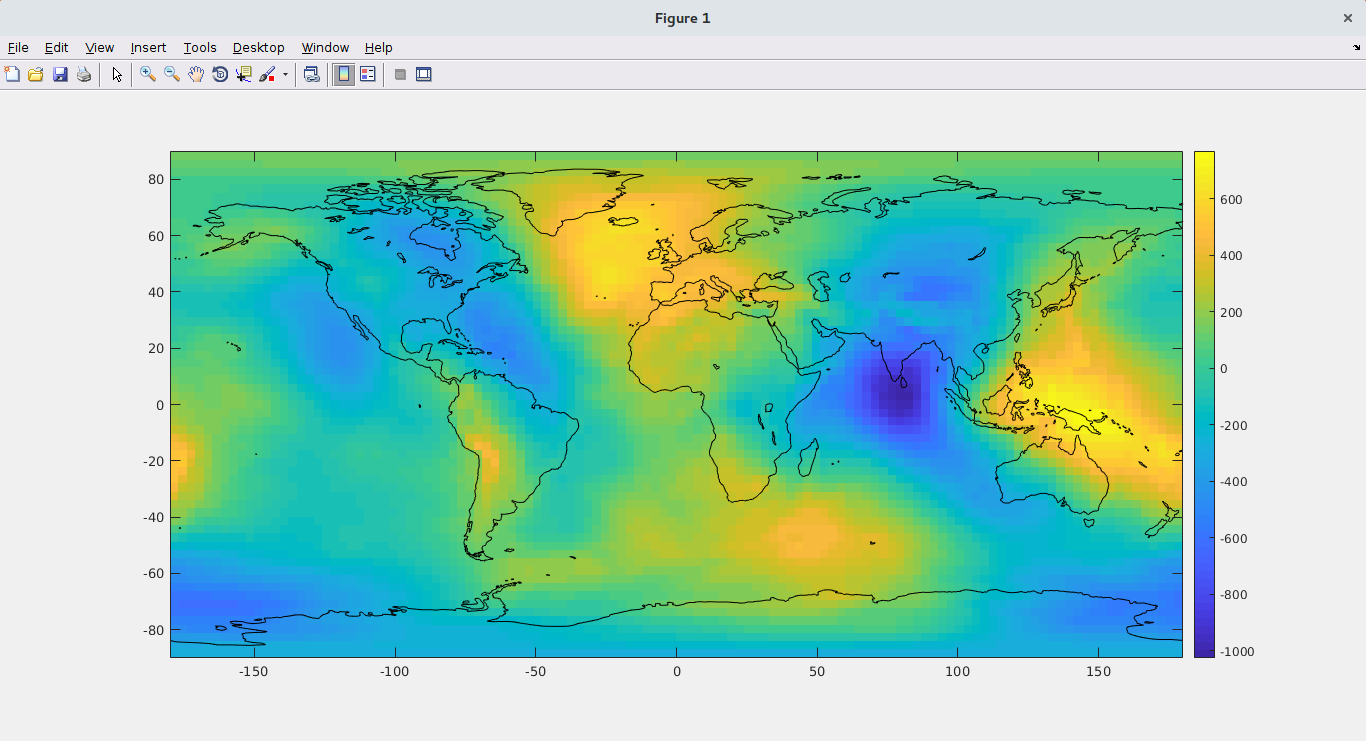
\includegraphics[scale=0.30]{DisturbanceField}
\newpage






\section{Analysis in spectral domain}
From Grace we get a set of real-valued SH-coefficients, complete to maximum degree L
Clm coefficients as matrix in the form\\
\[
\begin{bmatrix}
    l_{11}       & m_{12} & C_{13} & S_{1n} \\
    l_{21}       & m_{22} & C_{23} & S_{2n} \\
    \hdotsfor{4} \\
    l_{d1}       & m_{d2} & C_{d3} & S_{dn}
\end{bmatrix}
\]\\
% \[ 
% \,[l\quad m\quad C\quad S\quad [\,sigma_C\quad sigma_S]\,]
% \]
% write in matrix form using math mode
Using the function clm2sc we convert CLM format to SC format for further filtering analysis because it's easy to inspect error in SC format.
Then the SC-format stores the coefficients in the following $(L + 1)\times (2L + 1)$ matrix:\\

\[
\centering%
\begin{bmatrix}%
      &         &         &         & C_{00}   &         &         &             & \\
      & \epsilon&         & S_{11}  & C_{10}   &C_{11}   &         & \epsilon    & \\
      &         & S_{22}  & S_{21}  & C_{20}   & C_{21}  & C_{22}  &             & \\
      &         &\vdots{} &\vdots{} & \vdots{} &\vdots{} &\vdots{} &\ddots       & \\
      S_{LL}    &\cdots   & S_{L2}  & S_{L1}   & C_{L0}  & C_{L1}  & C_{L2}      &\cdots &C_{LL}
\end{bmatrix}%
\]\\
The upper left and right corners should be filled with zeros. For some \\ numerical purposes,
it could be handy though, to use a small number $epsilon$, e.g. $\epsilon = 10^{-20}$.
The name SC-format is chosen since the $S_{lm}$-coefficients are at the LHS and the $C_{lm}$-coefficients at the RHS of the matrix\\
$EXAMPLE: clm2sc\quad(\,clm,\, max_lm,\, 30, gcoef2sc,\, false\,)\,;$
%Using Sctriplot function SCTRIPLOT plots the triangles of SH coefficients stored in SC-format. If stored in CS format it is converted to SC-format before plotting.
%Plot the figure
% The sectorial and near sectorial terms above degree 60 are of a degraded quality as compared to other terms in all cases
\paragraph{\centerline{Triangular plot of $C_{lm}$ and  $S_{lm}$}}

\begin{figure}[ht]
\centering

%\includegraphics[scale=0.22]{Triangle}

\end{figure}


\newpage
\section{Spherical Harmonics}
\subsection{Visualising the spherical harmonics}
Visualising the spherical harmonics is a little tricky because they are complex and defined in terms of angular co-ordinates, ($\theta,\phi$).\\
One way is to plot the real part only on the unit sphere.We plotted it on
python using the $sph\_harm$ package available in $scipy$ module.
Following are the plots for corresponding l(degree) and m(order):
% plot the figures
Red area shows positive values while Blue area shows negative values.

\subsection{How  to get mass changes from GRACE?}
In principle:\\
1) Get a program for spherical harmonic grid synthesis.\\
2) Download GRACE Release 5 (”best”) coefficients from CSR or GFZ \\(max degree 60) monthly solutions.\\
3) Make average geoid coefficients for a period, e.g. 2003-2012\\
4) Make coefficient differences to average ($\Delta C_{lm}, \Delta S_{lm}$)\\
5) Evaluate surface mass grids by , put in convenient units and Plot the disturbing field plot but before that it needs some filtering to remove noises in the data. \\


\end{document}
